\documentclass{beamer}

\usepackage{cite}


\usetheme{metropolis}
% Customize to grayscale
\definecolor{mDarkGray}{RGB}{50,50,50}
\setbeamercolor{normal text}{fg=black, bg=white}
\setbeamercolor{frametitle}{bg=mDarkGray, fg=white}
\setbeamercolor{progress bar}{fg=mDarkGray, bg=lightgray}

\title{Plane Crash Fatality Modeling}
\author{Andreas Bogossian \& Markus Kruth}
\date{}

\begin{document}

\frame{\titlepage}



\begin{frame}{Number of crashes}
    \begin{figure}
        \centering
        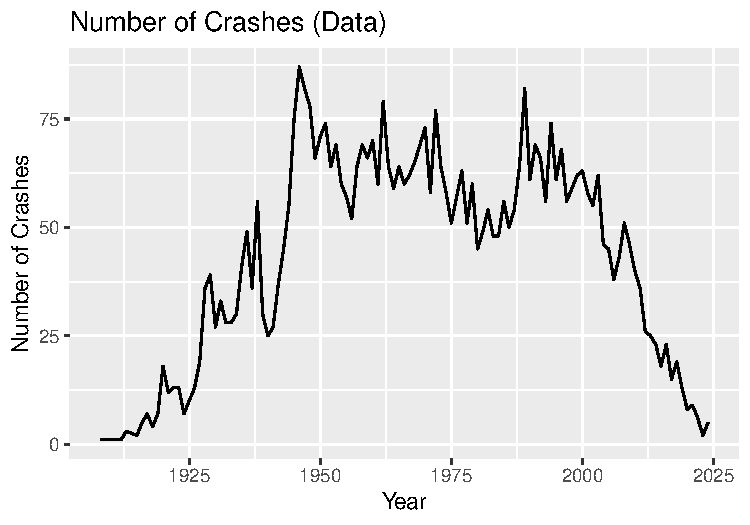
\includegraphics[width=1\linewidth]{figures/crashes-data.pdf}
        \label{fig:placeholder}
    \end{figure}
\end{frame}

\begin{frame}{Fatality Rate}

    Definition: the percentage of the people aboard that die.

    \begin{figure}
        \centering
        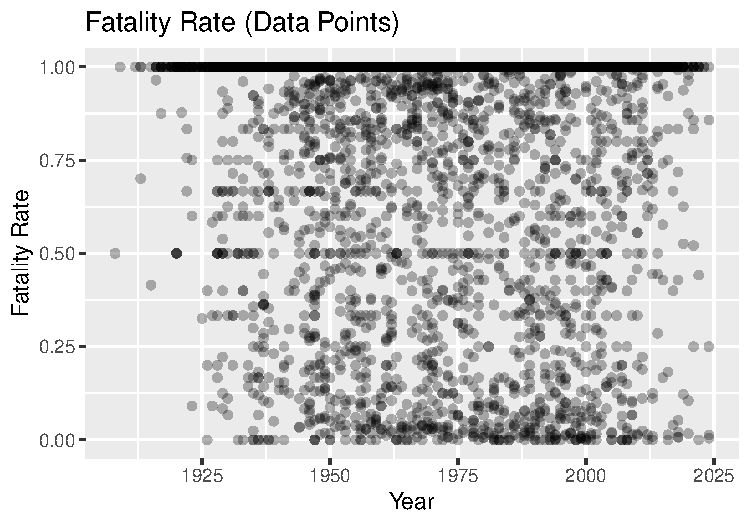
\includegraphics[width=\linewidth]{figures/fatality-rate-data.pdf}
        \label{fig:fatality-data}
    \end{figure}
\end{frame}

\begin{frame}{Fatality Rate (Trend)}
    \begin{figure}
        \centering
        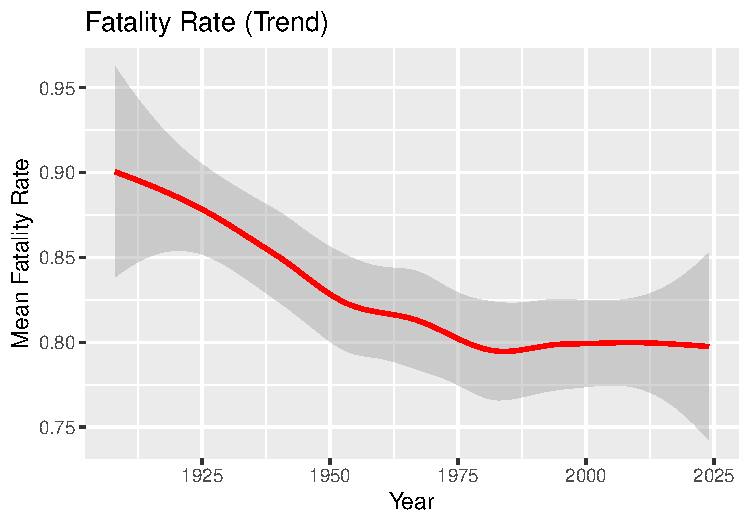
\includegraphics[width=\linewidth]{figures/fatality-rate-trend.pdf}
        \label{fig:fatality-trend}
    \end{figure}
\end{frame}

\begin{frame}{Research Question}
    \begin{itemize}
        \item Are some manufacturers making safer planes than others?
        \item If so, how much safer?
    \end{itemize}
\end{frame}

\section{Dataset}

\begin{frame}{Dataset}

    \begin{itemize}
        \item Dataset: All recorded airplane crashes since 1908 \cite{jogwums2023aircrashes}
        \item Columns of interest:
              \begin{itemize}
                  \item Number of people on board
                  \item Number of people that died
                  \item Date of the crash
                  \item Manufacturer of the crashed plane
              \end{itemize}
        \item Filters
              \begin{itemize}
                  \item year $\geq 1975$
                  \item manufacturer $\geq 10$ crashes
              \end{itemize}
    \end{itemize}


\end{frame}

\section{Models}

\begin{frame}{Models used}
    \begin{itemize}
        \item \textbf{Complete pooling model:} one shared fatality probability for all manufacturers.
        \item \textbf{No pooling model:} each manufacturer estimated independently.
        \item \textbf{Partial pooling model:} manufacturer effects vary but are partially pooled, giving the most reliable comparison.
    \end{itemize}
\end{frame}

\begin{frame}{Piors}

    For the priors we used weakly informative priors integrated with some information from the data.

    \begin{itemize}
        \item \(\alpha_0 \sim \mathcal{N}(1.4, 1)\)
        \item \(\beta_0 \sim \mathcal{N}(0, 0.5)\)
        \item \(\alpha_m,\beta_m \sim \mathcal{N}(0, 1)\)
    \end{itemize}


\end{frame}

\begin{frame}{Complete pooling model}

    \(y_i \sim \text{Binomial}(n_i, p_i)\) \\
    \(\operatorname{logit}(p_i) = \alpha_0 + \beta_0 \cdot year\_scaled_i\)

    \vspace{0.5em}

    \begin{itemize}
        \item \(\hat{R}=1.00\)
        \item Bulk ESS: $> 3000$
        \item Tail ESS: $> 2000$
        \item No divergences
    \end{itemize}

\end{frame}

\begin{frame}{Complete pooling model}

    \begin{figure}
        \centering
        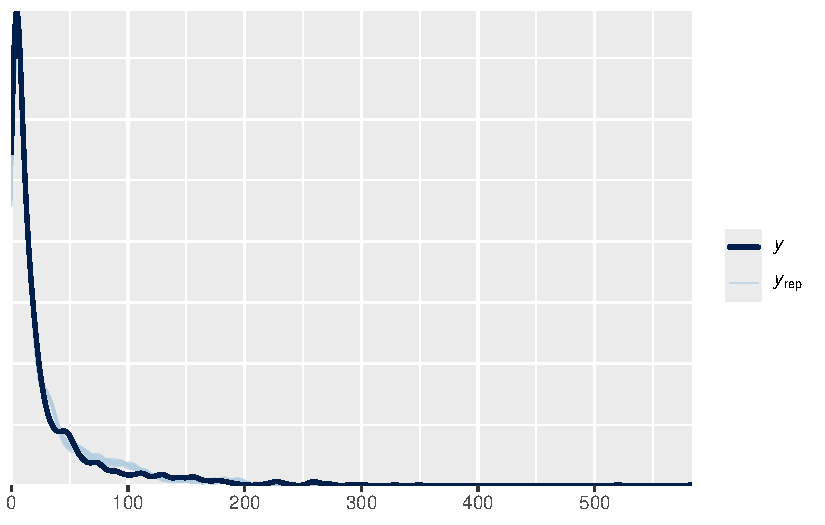
\includegraphics[width=\linewidth]{figures/complete_pool_ppcheck.pdf}
        \label{fig:complete-pooling-ppcheck}
    \end{figure}

\end{frame}



\begin{frame}{No pooling model}

    \(y_i \sim \text{Binomial}(n_i, p_i)\) \\
    \(\text{logit}(p_i) = \alpha_{m} + \beta_{m} \cdot year\_scaled_i\)

    \vspace{0.5em}

    \begin{itemize}
        \item \(\hat{R}=1.00\)
        \item Bulk ESS: $> 4200$ for all
        \item Tail ESS: $> 2600$ for all
        \item No divergences
    \end{itemize}

\end{frame}

\begin{frame}{No pooling model}

    \begin{figure}
        \centering
        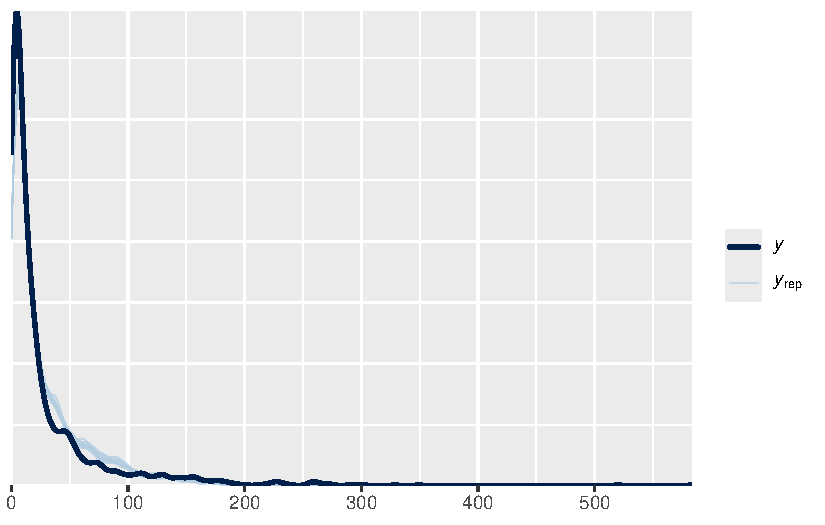
\includegraphics[width=\linewidth]{figures/no_pool_ppcheck.pdf}
        \label{fig:fatality-trend}
    \end{figure}

\end{frame}


\begin{frame}{Partial Pooling model}

    \(y_i \sim \text{Binomial}(n_i, p_i)\)
    \(\text{logit}(p_i) = \alpha_0 + \beta_0 \cdot year\_scaled_i + \alpha_{m} + \beta_{m} \cdot year\_scaled_i\)


    \begin{itemize}
        \item \(\hat{R}=1.00\) and \(\hat{R}=1.01\)
        \item No divergences
        \item Multilevel Hyperparameters ($\sigma_\alpha, \sigma_\beta, \rho$)
              \begin{itemize}
                  \item Bulk ESS $> 850$ \& tail ESS $> 1100$
              \end{itemize}
        \item Fixed effects ($\alpha_0, \beta_0$)
              \begin{itemize}
                  \item Bulk ESS $> 500$ \& tail ESS $> 950$
              \end{itemize}

    \end{itemize}

\end{frame}

\begin{frame}{Partial Pooling Model}
    \begin{figure}
        \centering
        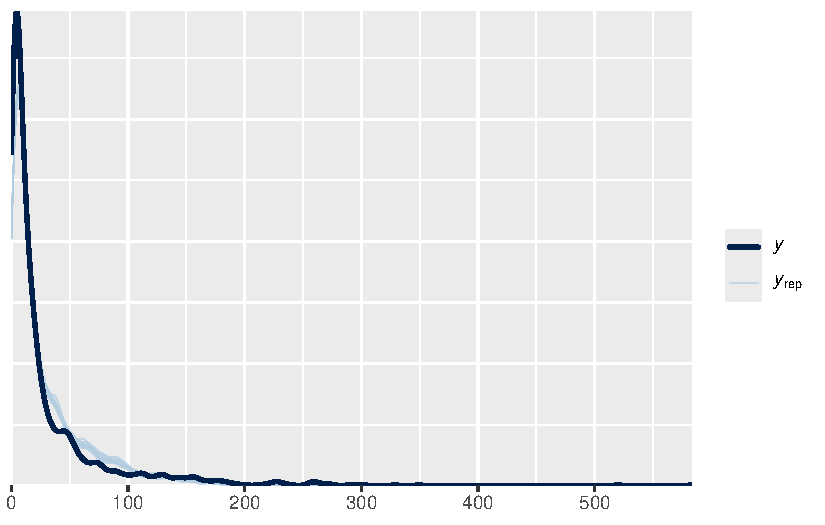
\includegraphics[width=\linewidth]{figures/no_pool_ppcheck.pdf}
    \end{figure}
\end{frame}

\section{Model Comparison}

\begin{frame}{Model comparison (LOO-CV)}

    \begin{table}[h]
        \centering
        \begin{tabular}{lrrr}
            \hline
            Model                 & elpd\_diff & se\_diff & $\left|\frac{elpd\_diff}{se\_diff}\right|$ \\
            \hline
            partial\_pool\_model  & 0.0        & 0.0      & --                                         \\
            no\_pool\_model       & -16.5      & 13.3     & 1.24                                       \\
            complete\_pool\_model & -1944.8    & 692.3    & 2.81                                       \\
            \hline
        \end{tabular}
        \caption{LOO-CV model comparison results}
        \label{tab:model_comparison_ratio}
    \end{table}

\end{frame}

\section{Conclusions}

\begin{frame}{Conclusions}

    \begin{itemize}
        \item Partial pooling and no pooling models perform the best \\
              $\Rightarrow$ Manufacturer level differences exist
        \item Models were unaffected from changes in priors \\
              $\Rightarrow$ Models not dependent on choice of priors
        \item Models were not capturing the variance of the original data (underdispersion) \\
              $\Rightarrow$ Due to fixed variance of binomial model (too small)
    \end{itemize}

\end{frame}



\begin{frame}[allowframebreaks]{References}
    \bibliographystyle{IEEEtran}
    \bibliography{references}
\end{frame}


\end{document}